\documentclass[a4paper,10pt]{article}
\usepackage[utf8]{inputenc}
\usepackage{amsmath}
\usepackage{amsfonts}
\usepackage{amssymb}
\usepackage{algorithm}
\usepackage{algorithmic}
\usepackage{graphicx}
\usepackage{tikz}
\usepackage{amsthm}
\graphicspath{{figures/}}
%opening
\title{Parallel computation of the trajectory of a Markov process}
\author{Jean-Michel Fourneau \and Maël Guiraud \and Yann Strozecki}
\newcommand{\cS}{\mathcal{S}}
\newcommand{\todo}[1]{{\color{red} TODO: {#1}}}
\renewcommand{\algorithmicrequire}{\textbf{Input:}}
\renewcommand{\algorithmicensure}{\textbf{Output:}}

 \newtheorem{theorem}{Theorem}
  \newtheorem{proposition}{Proposition}
\begin{document}

\maketitle

\begin{abstract}
In this short article, we describe several methods to compute the trajectory of a Markov process in parallel. 
Our algorithms rely on the fact that the states of the process are partially ordered. We explain under which assumption we can 
obtain a speedup using a parallel algorithm and we give experimental evidences that the method works better than sequential or classic parallel simulation.
\end{abstract}

\section{Introduction} %Ici le modèle + les références

Let $\cS$ be a finite set of states and let $f$ be a computable function from $\cS \times [0,1]$ to $\cS$. 
The aim of this short article is to propose practical methods to compute in parallel the sequence $T(s,x_1,\dots,x_n)= (s_0, \dots, s_n)$ where $s_i = f(s_{i-1},x_i)$ and $s_0 = s$. The elements $(x_0,\dots,x_n)$ are realizations of a sequence of independent and identically distributed random variables $X_0,\dots,X_n$. This models a random process on a finite set of states, which depends only on the current state, in other words a \emph{Markov process}.

In general,  $s_n$ depends on $s$ and all $x_i$'s and thus cannot be computed without reading all $x_i$'s,
which makes parallelization impossible in general. Hence, we consider additional structure on $\cS$ to make the problem tractable. The set $\cS$ is equipped with a partial order $\leq$ and it has a smallest element $\bot$ and a greatest element $ \top$. We assume that $f$ is monotone, that is if $s_1$ and $s_2$ are elements of $\cS$ such that $s_1 \leq s_2$ then for all $x\in[0,1],\, f(s_1, x) \leq f(s_2, x)$. Given a function $f$, a state $s$ and a sequence $x_0,\dots,x_n$ of realizations of $X_0,\dots,X_n$, we want to compute the sequence $T(s,x_1,\dots,x_n)$ when $\cS$ is a partially ordered set. We call this problem \textsc{PoTraSim}, for partially ordered trajectory simulation.  

In practice, the values $x_1,\dots,x_n$ are given by a pseudo random generator initialized by some random seed.
These values can be generated efficiently in parallel without changing their distribution and thus the distribution of the generated 
trajectories: An integer $k$ is chosen and the values $x_{ki}$ are generated using a pseudo random generator and a random seed, then in parallel a pseudo random generator is used to generate $x_{ki +1},\dots, x_{ki + k - 1}$ using $x_{ki}$ as a seed. When $ k = \sqrt{n}$, this computation uses a parallel time of $O(\sqrt{n})$. This efficent parallelization justifies our choice of considering the sequence $x_1,\dots,x_n$ as an input in the problem \textsc{PoTraSim}.

To formalize our parallel algorithms, we choose a simple PRAM model --exclusive read and exclusive write (EREW)-- with shared memory to neglect synchronization and communication problems (see~\cite{jaja1992introduction}). This simplification is reasonnable in a multicore machine, since in our algorithms we use very few concurrent accesses to only limited informations, which can be dealt with no or almost no locking. For a distributed computing point of view, the cost of communication is also relevant since it tends to dominate the computing time. Both contexts are investigated in our experimentations.


\todo{Expliquer ici ce qui s'est fait avant (avec moins de suppositions). Ce qui s'est fait en général avec des espaces d'états po (travail de JMF)
Expliquer ensuite nos contributions.}

\section{Parallel computation}

The main idea of the method is to divide the sequence $T$ of size $n$ into smaller intervals of $t$ states. If we know the initial state of each interval then we can compute the sequences of iterates independently. 
In the PRAM model, with an unbounded number of processors and zero cost of communication, it may be optimal to have $t$ small and independent from $n$, but in practice cores are a scarce ressource and we will set $n/t$ to a value related to the number of machines or cores avalaible.

\subsection{Two bounds}

In this section, we describe an algorithm which solves \textsc{PoTraSim} in parallel, that is given $s$, $x_1,\dots,x_n$ and an algorithm to compute $f$ as inputs, it produces the sequence  $T(s,x_1,\dots,x_n)$. We fix a $t$, the size of an interval and we denote by $k = n/t$ the number of intervals. We store the status of each interval $j$ in a variable $status_j$ whose value can be  $\textsc{ToCompute}$, $\textsc{Computed}$ or $\textsc{Done}$. We also store for each $0 \leq j < k$ the states $s_j^{min}$ and $s_j^{max}$ which are lower and upper bound on the real trajectory at the beginnig of the $j$th interval. In all the algorithms we describe, the following invariant is true: $s_j^{min} \leq s_{j*t} \leq s_j^{max}$.
 
Let us now describe the execution of the algorithm. At the beginning, the status of each interval is $\textsc{ToCompute}$, and the lower bounds are set to the minimal elements and the upper bounds to the maximal except for the first. For all $0 < j < k$, $status_j = \textsc{ToCompute}$,  
$s_j^{min} = \bot$ and $s_j^{max} = \top$. Moreover $status_0 = \textsc{ToCompute}$ and $s_0^{min} = s_0^{max} = s$.

While there is a free processor $P$ and a $j$ such that $status_j = \textsc{ToCompute}$, the index $j$ is selected. The variable $status_j$ is then set to $\textsc{Computed}$ and the processor $P$ computes the two sequences $T(s_j^min,x_{jt},\dots,x_{(j+1)t})$ and $T(s_j^max,x_{jt},\dots,x_{(j+1)t})$. 
The last value of the two computed sequences, let us denote them by $s_min$ and $s_max$, are then compared to the bounds of the next interval if there is one.  
 If $s_min > s_{j+1}^{min}$ or $ s_max < s_{j+1}^{max}$ then better bounds have been found and $P$ sets $s_{j+1}^{min} = s_min$, $s_{j+1}^{max} = s_max)$ and $s_{j+1} = \textsc{ToCompute}$.
Finally, when a processor simulate the interval $j$ and at the beginning $s_j^{min} = s_j^{max}$, the result of the simulation is stored as a part of the trajectory and $s_j = \textsc{Done}$ at the end.
The algorithm we just described is called \textsc{Speculative Sandwich} and we give its pseudocode in Figure~\ref{fig:par_sandwich}.


 	\begin{algorithm}[H]
 	\caption{Speculative Sandwich}
 	\label{fig:par_sandwich}
 	\begin{algorithmic}
	\REQUIRE Size of the intervals $t$
 	\STATE // {\em Initialisation}
	\FOR{ $i <$ min(nb\_machines, nb\_inter-1) }
	\STATE Send $I_{j+1}$ to the server $i$
	\ENDFOR
	\STATE // {\em Main loop}
 	\WHILE{ All the intervals are not $\textsc{Done}$}
	\STATE Wait for a server to answer the results of $current\_interval$
	\IF{The server was computing a trajectory}
	\STATE set $I_{current\_interval}$ to $\textsc{Done}$
	\ENDIF
	\IF{$f^t(s_{current\_interval}^{min}) > s_{current\_interval+1}^{min}$ or $f^t(s_{current\_interval}^{max}) < s_{current\_interval+1}^{max}$ // {\em Better bounds have been found} }
	\STATE $s_{current\_interval+1}^{min} = f^t(s_{current\_interval}^{min})$
	\STATE $s_{current\_interval+1}^{max} = f^t(s_{current\_interval}^{max})$
	\STATE set $I_{current\_interval}$ to $\textsc{ToCompute}$
	\ENDIF
	\STATE next\_interval $\leftarrow$ search the first interval which is to  $\textsc{ToCompute}$
	\IF{ $s_{next\_interval+1}^{min} = s_{next\_interval+1}^{max}$ // {\em The bounds are coupled} }
		\STATE Wait a trajectory for $I_{next\_interval}$
	\ELSE
		\STATE Wait some bounds for $I_{next\_interval}$
	\ENDIF	
		\STATE Send $s_{next\_interval+1}^{min} and s_{next\_interval+1}^{max}$ to the current server
	\ENDWHILE
 
 	\end{algorithmic}
 	\end{algorithm}
 
 
 \begin{theorem}\label{th:alg_ok}
  \textsc{Speculative Sandwich} solves the problem \textsc{PoTraSim}. 
  \end{theorem}
  
\begin{proof}
First, we prove that \textsc{Speculative Sandwich} terminates and always compute the right answer.
Recall that we have stated that for all $j$, $s_j^{min} \leq s_{j*t} \leq s_j^{max}$. We can prove that 
this is true during all the algorithm by induction on the computation time. Indeed, $s_j^{min}$ and $s_j^{max}$ are changed when a simulation from $s_{j-1}^{min}$ and $s_{j-1}^{max}$ find tighter bounds. By induction hypothesis $s_{j-1}^{min} \leq s_{(j-1)*t} \leq s_{j-1}^{max}$ since the have been computed before. The monotony of $f$ guarantees that $j, s_j^{min} \leq s_{j*t} \leq s_j^{max}$. This guarantee that when $s_j^{min} = s_j^{max}$, the trajectory we simulate is correct. 

Let us prove that the when the algorithm stops it has computed all the trajectory. Assume for the sake of contradiction that the algorithm stops and that at least an interval with status $\textsc{Computed}$ and let 
$j$ the smallest index such that $status_j = \textsc{Computed}$. The interval $j>0$ since $status_0 = \textsc{Done}$ because $s_0^{min} = s_0^{max} = s$. Hence $j-1$ is positive and $status_{j-1} = \textsc{Done}$ by definition. But then \textsc{Speculative Sandwich} has updated the bounds $s_j^{min}$ and $s_j^{max}$ to $s_{jt}$ after the last simulation of the interval $j-1$. As a consequence \textsc{Speculative Sandwich} must have simulated the interval $j$ and marked it $\textsc{Done}$, a contradiction.

Finally let us prove that \textsc{Speculative Sandwich} terminates. 
To do that, it is enough to remark that each time a new interval is simulated,
it implies that the beginning bounds are tighter. Since the number of states is finished,
it implies that at some points the bounds are equal for each interval and the interval is marked $\textsc{Done}$.
\end{proof}


Remark that the way we select an index $j$ when there are several $status_j$ equal to $\textsc{ToCompute}$ is not specified. Each policy to select it gives rise to a different implementation of the algorithm \textsc{Speculative Sandwich}. Note that if we have an unbounded number of cores, we can always affect each 
avalaible interval to a different processor, therefore the policies are all the same. Hence they make sense in a context where the number of processors is limited.

We propose two different policies. 
The first is the \textsc{Ordered} policy: choose the avalaible interval with the smallest index. 
The second policy is called \textsc{Balanced} as we try to make the processors work on all parts of the trajectory more evenly. The $k$ intervals of size $t$ are grouped in $l$ larger meta-interval and 
we store how many intervals have been simulated in each meta interval. Then we select an avalaible interval
in the meta-interval with the less computed intervals. If there are several such intervals, we chose the one with the smallest index. 

For different policies, we would like to have a guarantee on the running time of  \textsc{Speculative Sandwich}. In particular, we would like it to be faster than the sequential time to solve \textsc{PoTraSim}.

\begin{proposition}
 \textsc{Speculative Sandwich} with policy \textsc{Ordered} solves \textsc{PoTraSim} in parallel time $Kn$ where $K$ is a bound on the time to compute $f$.
\end{proposition}
\begin{proof}
We prove that by induction on the time to simulate correctly the first $j$ intervals. 
Assume a processor $P$ has just finished to compute a sequence so that the first $j$ intervals
are correctly simulated in a time $T$ less than $Kjt$ by induction hypothesis. There is a time less or equal to $T$, such that a processor has finished the simulation of the interval $j-1$ and its status has been set to $\textsc{Done}$. Then by construction of \textsc{Speculative Sandwich}, the interval $j$ had its status set to $\textsc{ToCompute}$ and $s_j^{min} = s_j^{max}$ before time $T$.
If $status_j =  \textsc{Computed}$, by the previous remark, the interval is being 
simulated with the correct starting bound and will finish in less than $Kt$ time.
If $status_j =  \textsc{ToCompute}$, since the processor $P$ is free, it will simulate the interval $j$, since the \textsc{Ordered} select the smallest avalaible interval. This simulation will be finished in less than $Kt$ time. Thus the $j+1$ first intervals will be simulated in time less than $T + Kt \leq K(j+1)t$, which proves the induction.
\end{proof}

We have thus proved that the \textbf{Ordered} policy is always as fast as the sequential algorithm.
It would be interesting to understand when it is faster and by how much. 
If at some point of the algorithm, we have  $x_j^{min} = x_j^{max}$, we say that the 
two sequences are \textbf{coupling} on the interval $j$. If this phenomena happens frequently, the speed-up can be important. 

\begin{proposition}
 Let $f$ be such that 
\end{proposition}

For instance, in the best case, we have a coupling on each interval the first time it is simulated, then the sequential time is bounded by $O(ct)$.
% 
% Let us now consider the ordered policy.
% 






\subsection{A simple lockless implementation}

We can slightly improve the algorithm \textsc{Balanced Parallel Sandwich}.
First we make it simpler by cutting $[n+1]$ into $l$ intervals if we have $l$
processors, that is at first intervals and meta-intervals are the same. Then when a processor
a processor has correctly simulated its interval, we cut the remaining interval to simulate into 
intervals of similar sizes and affect one processor to each one.

\subsection{One bound}
\label{sec:onebound}

\todo{description of the algorithm and complexity bounds}

\section{Experimental evaluations}

\subsection{Settings}

\todo{Mettre ici la description de la chaîne et des outils communs}

\subsection{Multicore machine}

Closer to the abstraction of the previous part.
Mettre aussi les optimisations pour ce cas (on ne recalcule pas après couplage).


\subsection{Distributed computing}

Dire pourquoi ça se passe pas trop mal en distributed computing. 
Expliquer qu'on ne va pas envoyer la trajectoire (pas souvent utilisé en pratique) et qu'on va faire gaffe au temps de transfert. Remark that all processors do the simulation using only their private memory and the two states at the beginning of the interval. This scheme is thus reasonably adapted to a distributed computing environment where the cost of transmitting information between processors is high. 

\subsection{Random process}
\label{sec:randomproc}
The random process we use in our experiments is the following one. We have a system composed of $m$ finite queues of capacity BUFF\_MAX in tandem. A queue is characterized by its number of client $C_i$.  For each queue $i$, three events can occur:
\begin{itemize}
\item An arrival; $C_i$ is increased by one, if it is not already to BUFF\_MAX.
\item A service; if there is at least one client in $i$, a client leave the queue $i$ and goes in the queue $i+1$. $C_i$ is decreased by one and $C_{i+1}$ is increased by one. If $C_{i+1}$ is equal to BUFF\_MAX, the client is lost.
\item A departure: the client leave the system. The number of client of the queue is decreased by one if $C_i >0$.

\end{itemize}

For the queue $i$, every event have a probability denoted by respectively $a_i$, $s_i$ and $d_i$. The last queue has no service, thus $s_m = 0 $. There is thus a total of $3m-1$ different events that can change the system.


The sequence that we want to parallelize is a succession of drawing of one of those $3m-1$ events. Every event is drawn randomly, following a pseudo random generator. 

In the following experiments, the parameters $a_i$, $s_i$ and $d_i$ of the queues are set by the following rules:
\begin{itemize}
\item $P = 0.75$
\item $\mu = 300$
\item load = $1.1$
\item $a_0 = \mu \times $load
\item $a_i = (1-P) \times a_0, i \in [1:m]$
\item $s_i = P \times \mu, i \in [0:m]$
\item $d_i = (1-P) \times \mu, i \in [0:m]$
\end{itemize}
All those probabilities are then normalized such that $\sum\limits_{i=0}^m a_i + s_i + d_i = 1$.

With those parameters, every queue have an average load of $1.1$. This load has been experimentally calculated as the load for which the coupling time of the two bounds in the largest.

\begin{figure}[h]
 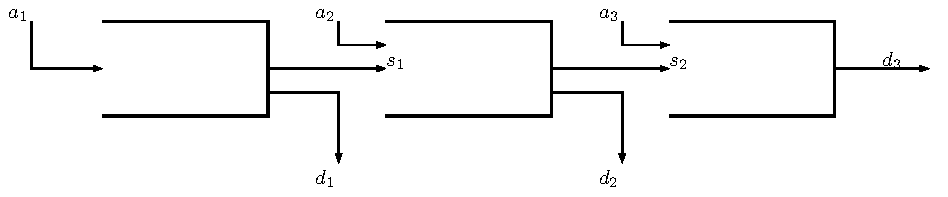
\includegraphics[scale=0.75]{tandem.pdf}
 \caption{A system with 3 queues}
\end{figure}

\subsection{Hardware and software used}

\subsection{Experimental settings}

Our experimentations are made with the following set-up.
The main program run on a MacBook Air, with a $2.2$ GHz Intel Core i$7$, and $8$ Go of RAM DDR$3$ at $1600$ MHz. The operating system of the machine is macOS High Sierra v$10.13.1$. The source code is compiled with  gcc version $7.1.0$ (Homebrew GCC $7.1.0$ -- without-multilib).

The simulations of each interval are dispatched on up to $7$ Raspberry Pi $3$ , Model B, with $1GB$ of RAM. Their operating system is  Raspbian GNU/Linux $8.0$, installed on a micro SD card element$14$ with a size of $8$GB. The source code is compiled with gcc version $4.9.2$ (Raspbian $4.9.2-10$). All the machines are connected to a local network through an HP $14$-$10$ $8$G switch.

<<<<<<< HEAD
All the machines are connected to a local network through an HP $14$-$10$ $8$G switch. 

During our experiments, we use the socket with the protocol TCP/IP to allow the servers and the master to communicate. All the machines were wired to a local network without access to any external networks. The source code of the simulation is written in C and available on the webpage of the authors. 
\todo{lien vers site yann avec code}

\subsection{Network impact}
\label{sec:networkimpact}
Since our network uses a local network with TCP/IP, one must investigate the cost of the network in our simulations. 
In our source code, we fixed the size of a standard master/server message to 24 integers and the size of the server/master messages depends of the number of queues in the simulation. One must focus on the cost of sending a trajectory, which is by far the largest message, indeed, the size of a trajectory is equal to $t \times m$($t$ is the size of the interval, and $m$ is the number of queues). On the following experiment, we tried to compare the evolution of the cost of the computing time and the network cost for different number of queues going from 1 to 10. We arbitrary set the size of the interval $t$ to $10,000$, which is a good order of magnitude considering the following experiments. The points on fig|~\ref{fig:example} are some average times computed on 100 different simulations.

\begin{figure}[h]
\centering
 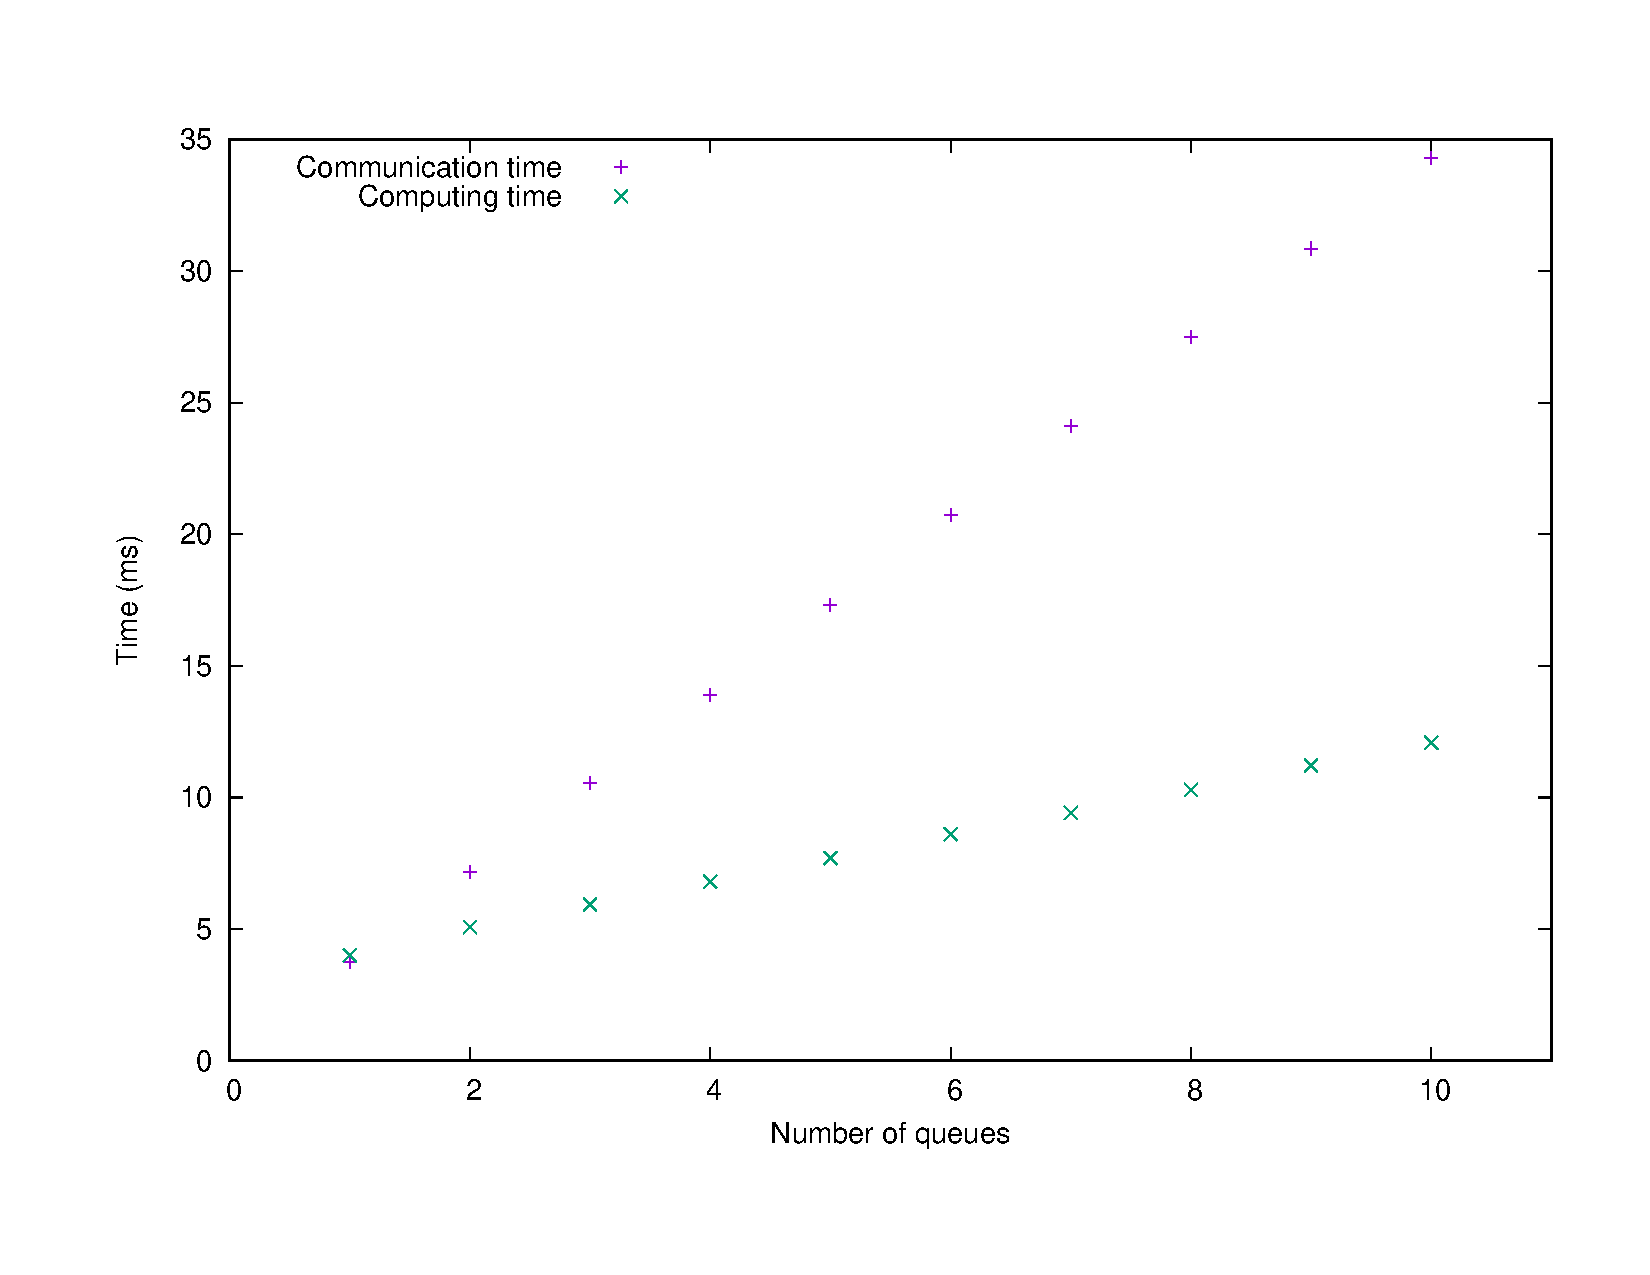
\includegraphics[scale=0.45]{time_traj.pdf}
 \caption{Evolution of the computing and communication time of a trajectory of $10,000$ events}
\end{figure}

As we can see, both the communication an computing times of a trajectory increases linerarly with the number of queues, but the communication time is increasing faster. A linear regression allowed us to calculate the slope of those two point clouds; the slope of the communication time is $3.390585$ while the slope of the computing time is only of $0.885585$. Both of those two correlations coefficients are greater $0.999$. Thus, to avoid an over domination of the network time, which would hide every interesting results, in the following experiments, we will consider a little number of queues in tandem.

\subsection{Algorithm performance evaluation}
We now want to measure the performance of the \textsc{Smallest Parallel Sandwich} and the \textsc{Balanced Parallel Sandwich}, compared to the One bound algorithm (cf sec~\ref{sec:onebound}). In the following experiment we thus take a random process with $5$ queues, which allows us to have a reasonable amount of computation in the servers, and a not too high $\frac{ \textrm{Network time} }{\textrm{Computing time}}$ ratio. In order to choose the size $n$ of the simulation, we made an upstream experiment to determine the average time between the coupling of the two bounds, for two queues, with the parameters we give in sec~\ref{sec:randomproc}. Thus, this average coupling time is to $28,049$, calculated over $100$ simulations.

\subsubsection{Long simulation}
We first want to look at the behavior of our algorithms in a simulation in which there is an high probability to have a coupling during the computing of a single interval. We then set the size of the simulation to $n = 210,000$. Fig.~\ref{fig:interslong} and ~\ref{fig:timelong} show the results of respectively, the average sum of the lengths of the intervals computed, and the average total time if simulation in regard of the number of intervals, over $100$ instances. By the way, the size of the interval directly depends of the number of intervals. The total size of the simulation is always the same, that is, $210,000$. We used $7$ servers in those experiments.

\begin{figure}[H]
\centering
\label{fig:interslong}
 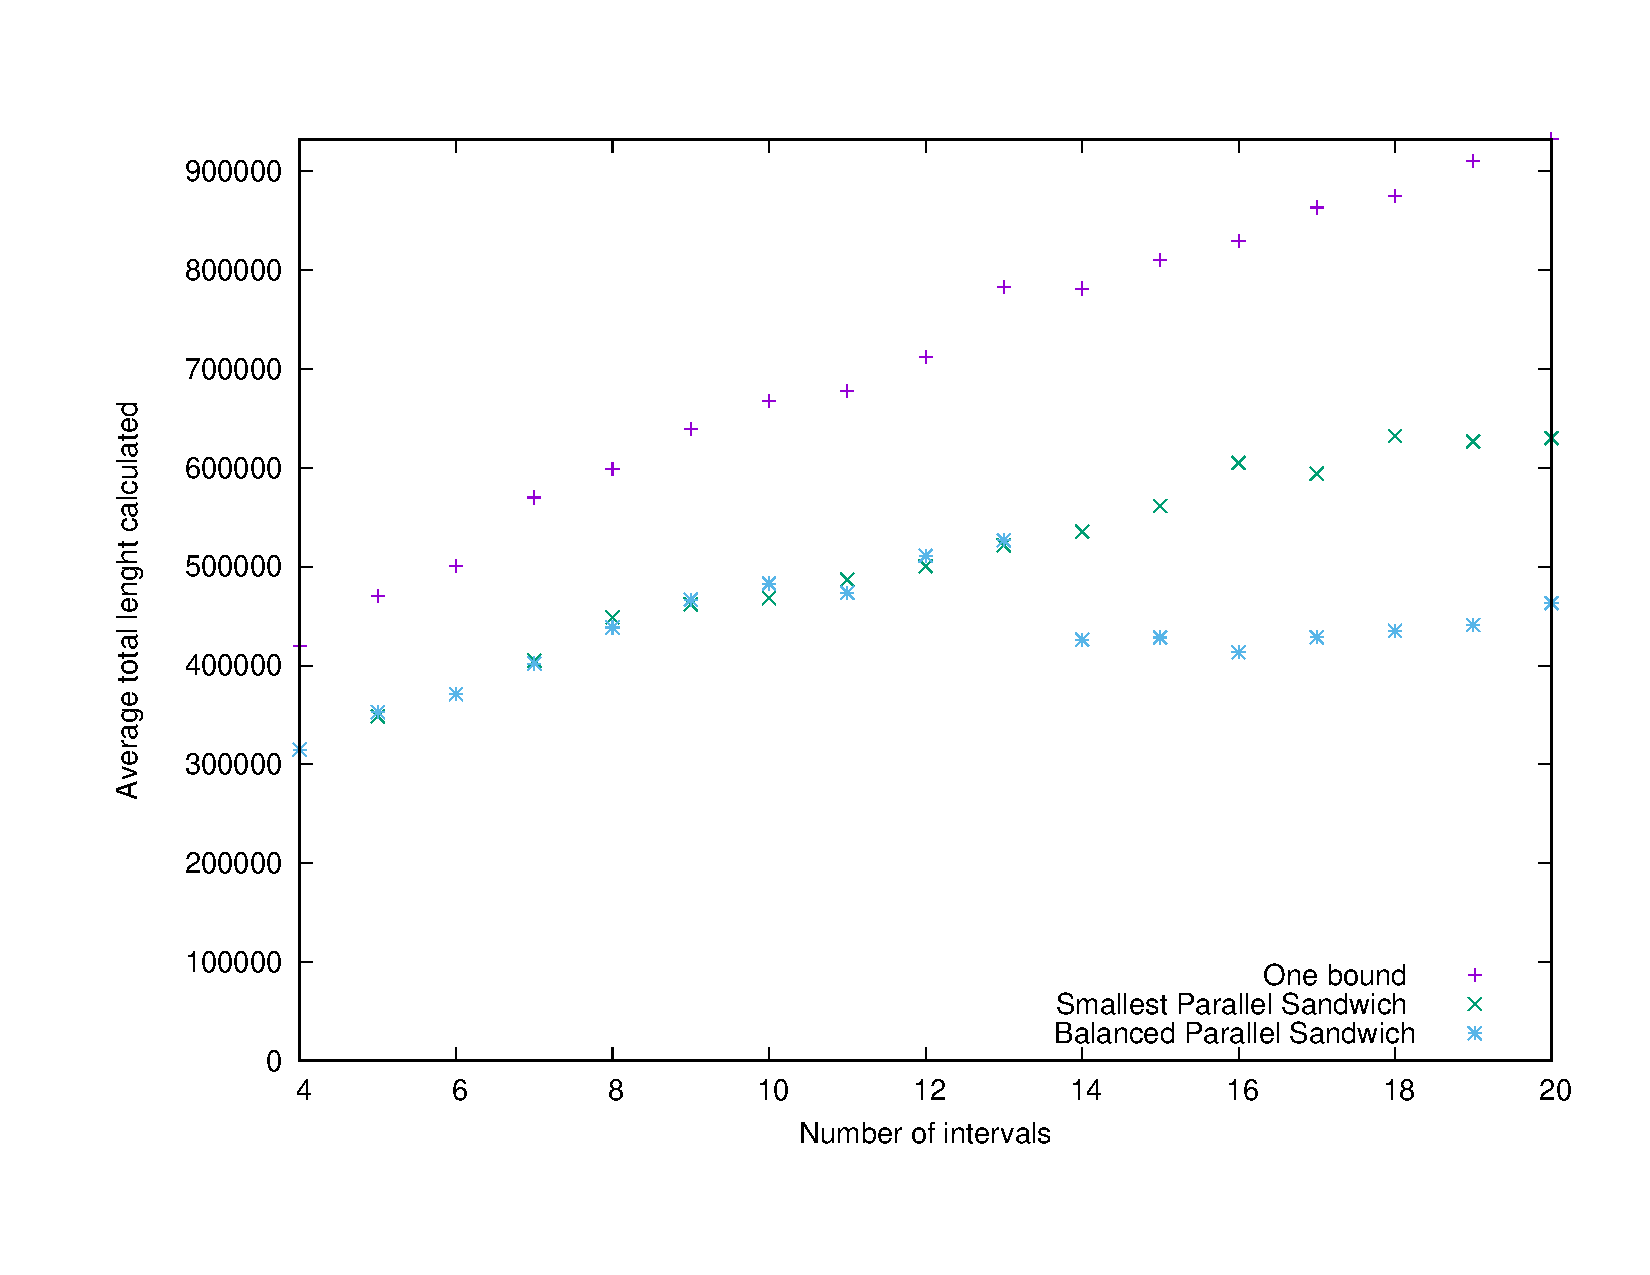
\includegraphics[scale=0.45]{interslong.pdf}
 \caption{Evolution of the average of the sum of the lengths of the intervals computed for $100$ simulations of $210,000$ events.}
\end{figure}

\begin{figure}[H]
\centering
\label{fig:timelong}
 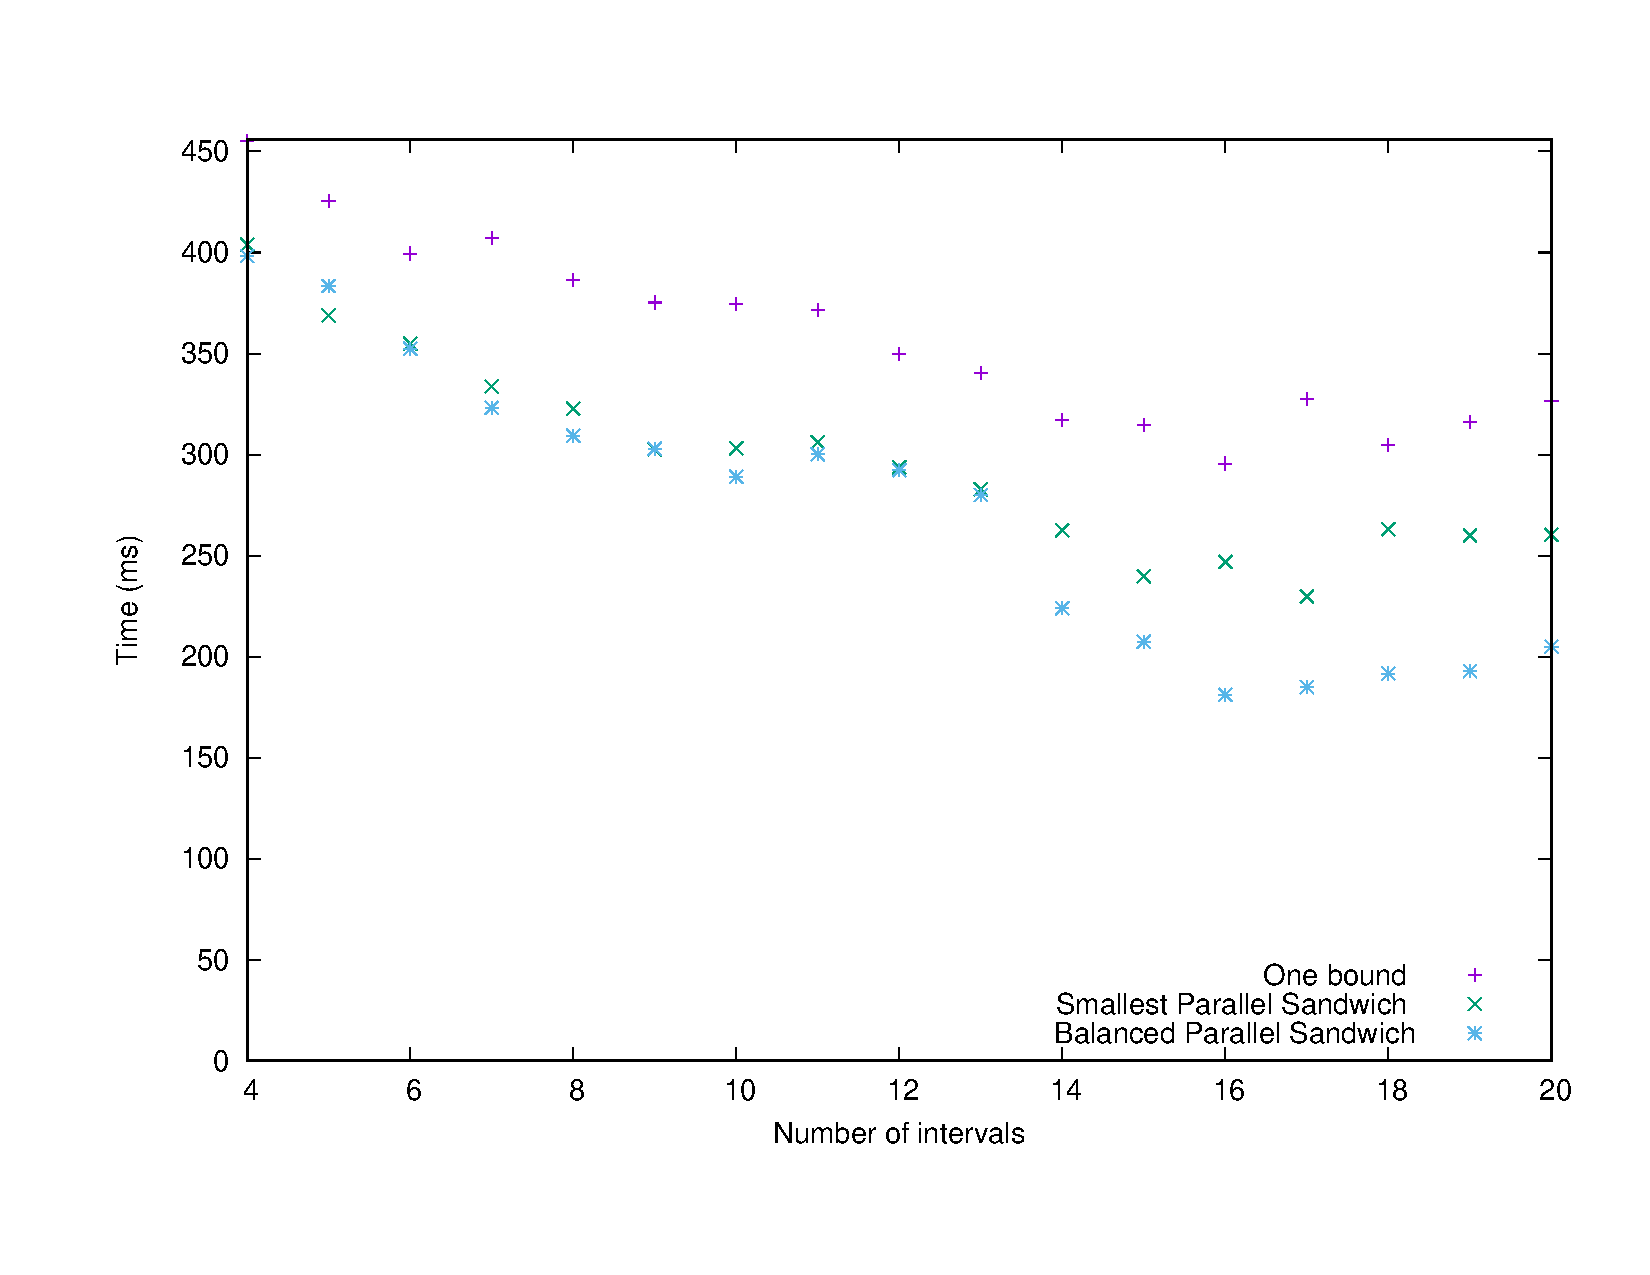
\includegraphics[scale=0.45]{timelong.pdf}
 \caption{Evolution of average for $100$ simulations of $210,000$ events.}
\end{figure}


First, we remark that the \textsc{Smallest Parallel Sandwich}  and the \textsc{Balanced Parallel Sandwich} are always better than the One Bound algorithm. The weak increasing trend for One Bound and \textsc{Smallest Parallel Sandwich} on fig.~\ref{fig:interslong} might be due to the decreasing probability of coupling in one interval when the number of intervals increases. Nevertheless the \textsc{Balanced Parallel Sandwich} seems to have a different behavior after an undetermined threshold. We will study this phenomenon later.

\todo{pas vraiment en fait, j'utilise le fait que il y ait ce point du rupture pour comparer les performances en fonction du nombre de servers mais je ne sais pas du tout pourquoi ca fait ca??}

In contrast to those results, as we can see on fig.~\ref{fig:timelong} , it looks like having few long intervals is more expensive in time than having more shorter intervals. This might be due to the network. Indeed, as we observed in the results of sec.~\ref{sec:networkimpact}, the more the interval is long, the more network increases. Moreover, the experiment in sec.~\ref{sec:networkimpact} were made on a single server communicating with the master. Here, we have 7 servers which probably create some contention, and thus, some additional latency.
On a single processor, the average time on $100$ simulations for $210,000$ events is to $162.13$ ms.

To make sure that the network is dominating the simulation time, we investigate the activity of the servers during the experiments. Fig.~\ref{fig:servers} shows the average repartition of the computation, network and waiting time of the servers, during the previous experiments, for the computation of the \textsc{Balanced Parallel Sandwich} simulations.


\begin{figure}[H]
\centering
\label{fig:servers}
 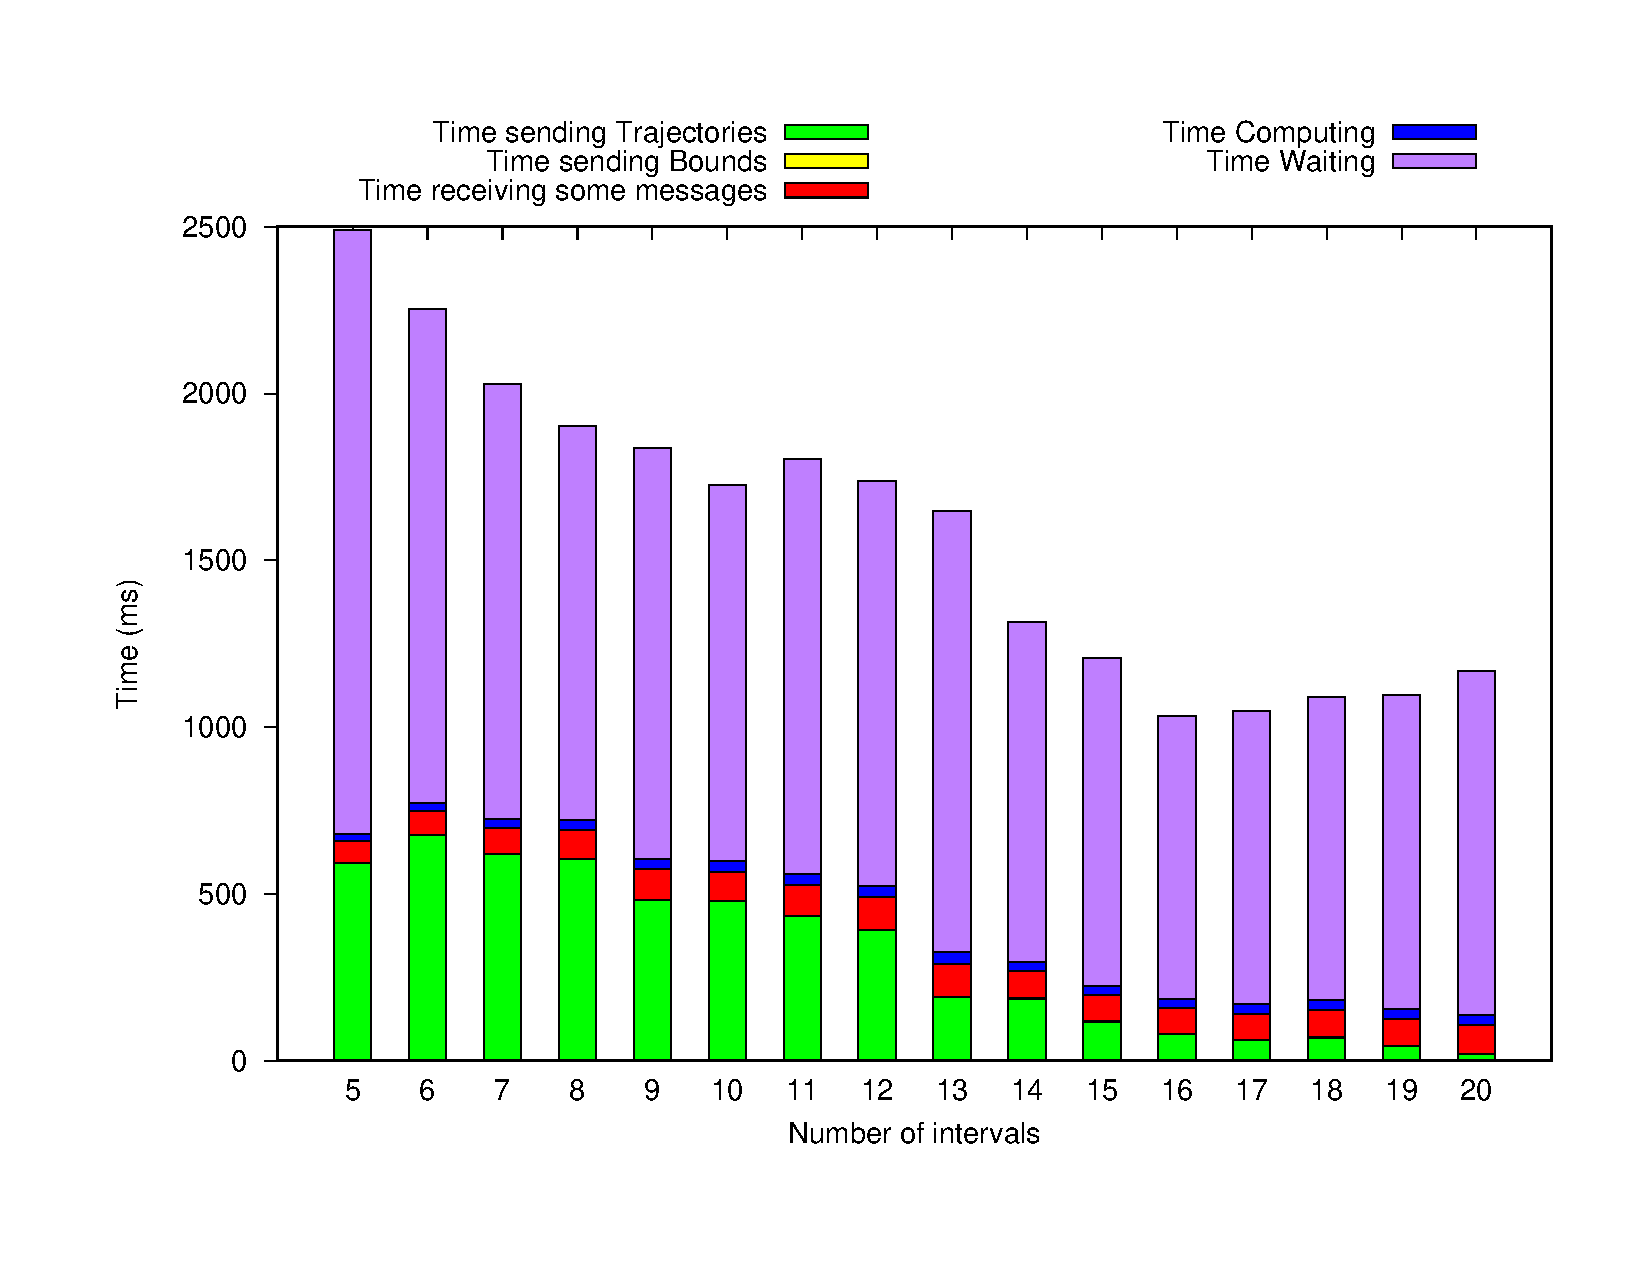
\includegraphics[scale=0.45]{server.pdf}
 \caption{Repartition of the activities of the processors during the simulation.}
\end{figure}

First, we can see that, the most of the time, the servers are waiting for something to do. Since the master algorithm is not very complicated, we suppose that the network highly slows the communication between the master and the servers. The rest of the time, the servers are mainly computing some network operations (sending, receiving).
\subsubsection{Short simulation}
We then tried to look if there is a difference when the simulation is short. The following experiment are made with exactly the same parameters than upward, except the simulation length, which is now of $30,000$. In this situation, the probability of coupling is very low.

\begin{figure}[H]
\centering
\label{fig:intersshort}
 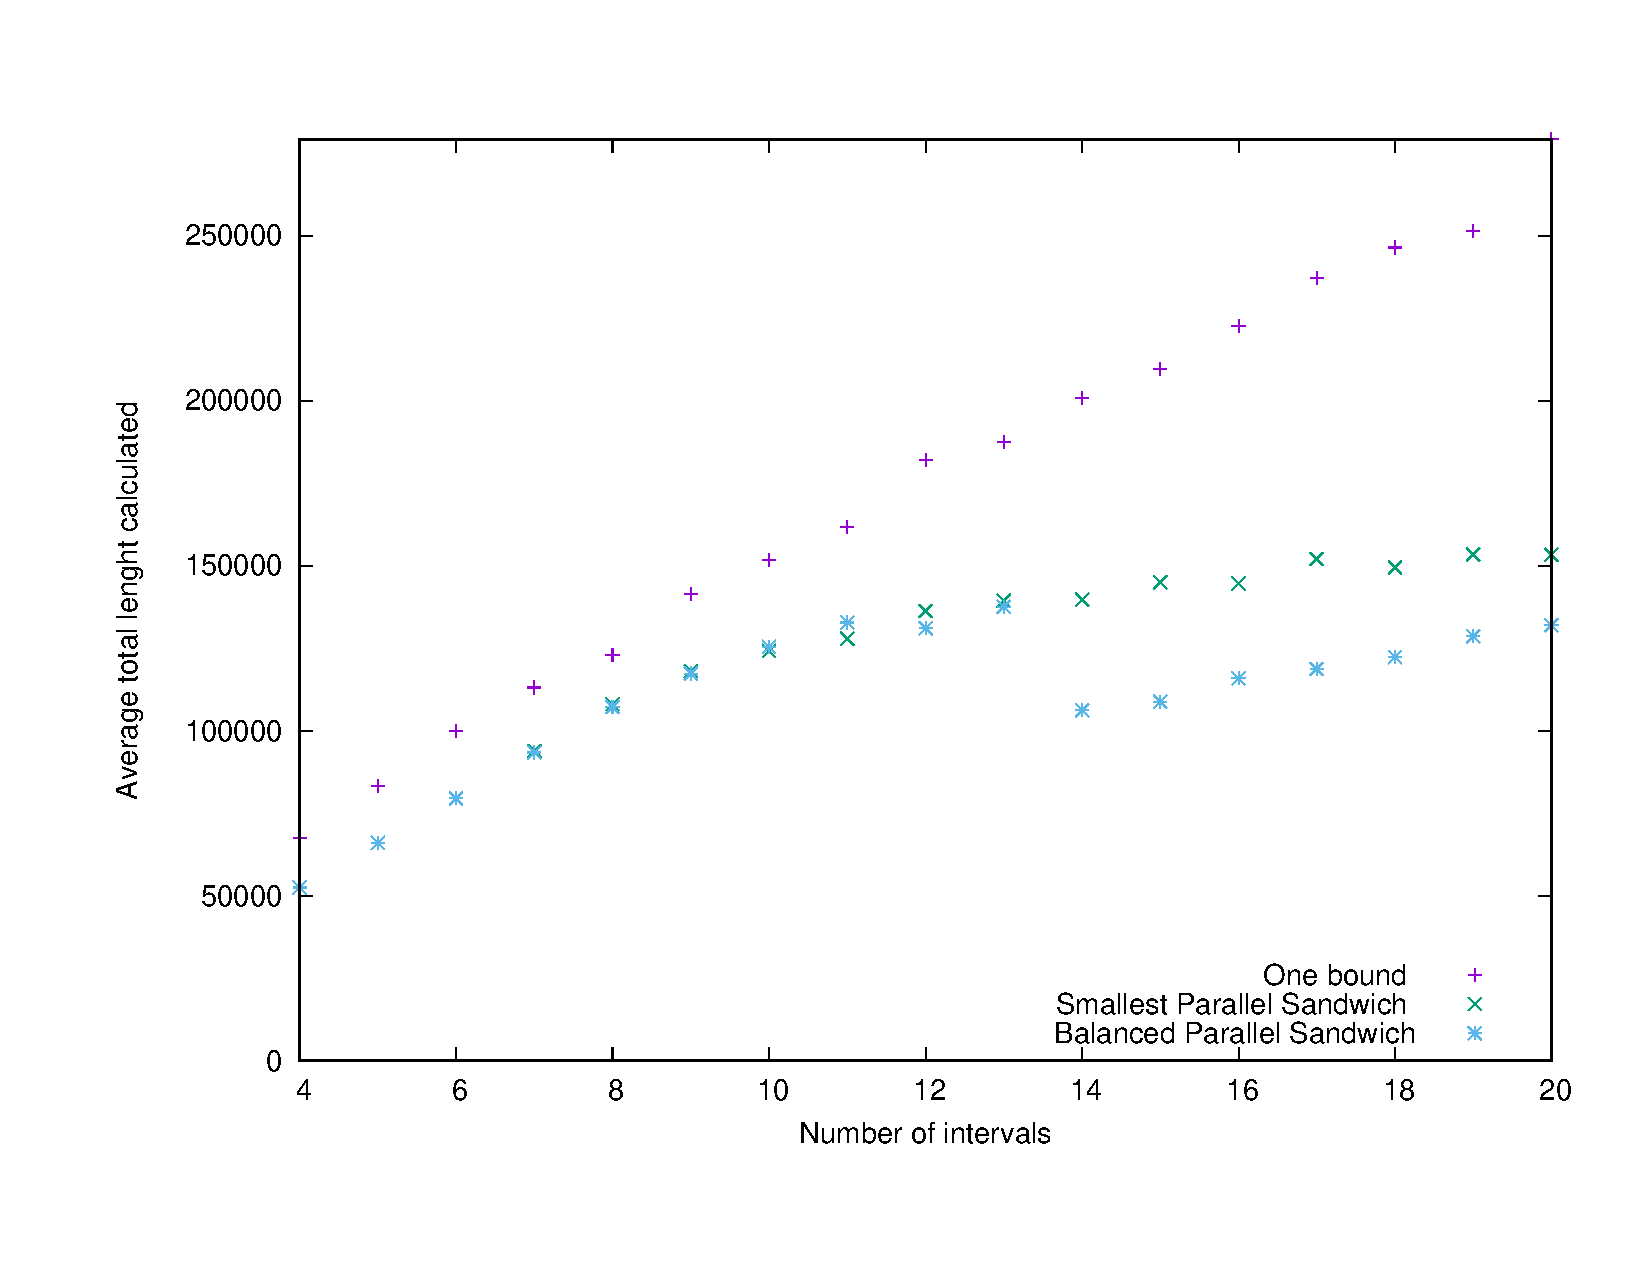
\includegraphics[scale=0.45]{intersshort.pdf}
 \caption{Evolution of the average of the sum of the lengths of the intervals computed for $100$ simulations of $30,000$ events.}
\end{figure}

\begin{figure}[H]
\centering
\label{fig:timeshort}
 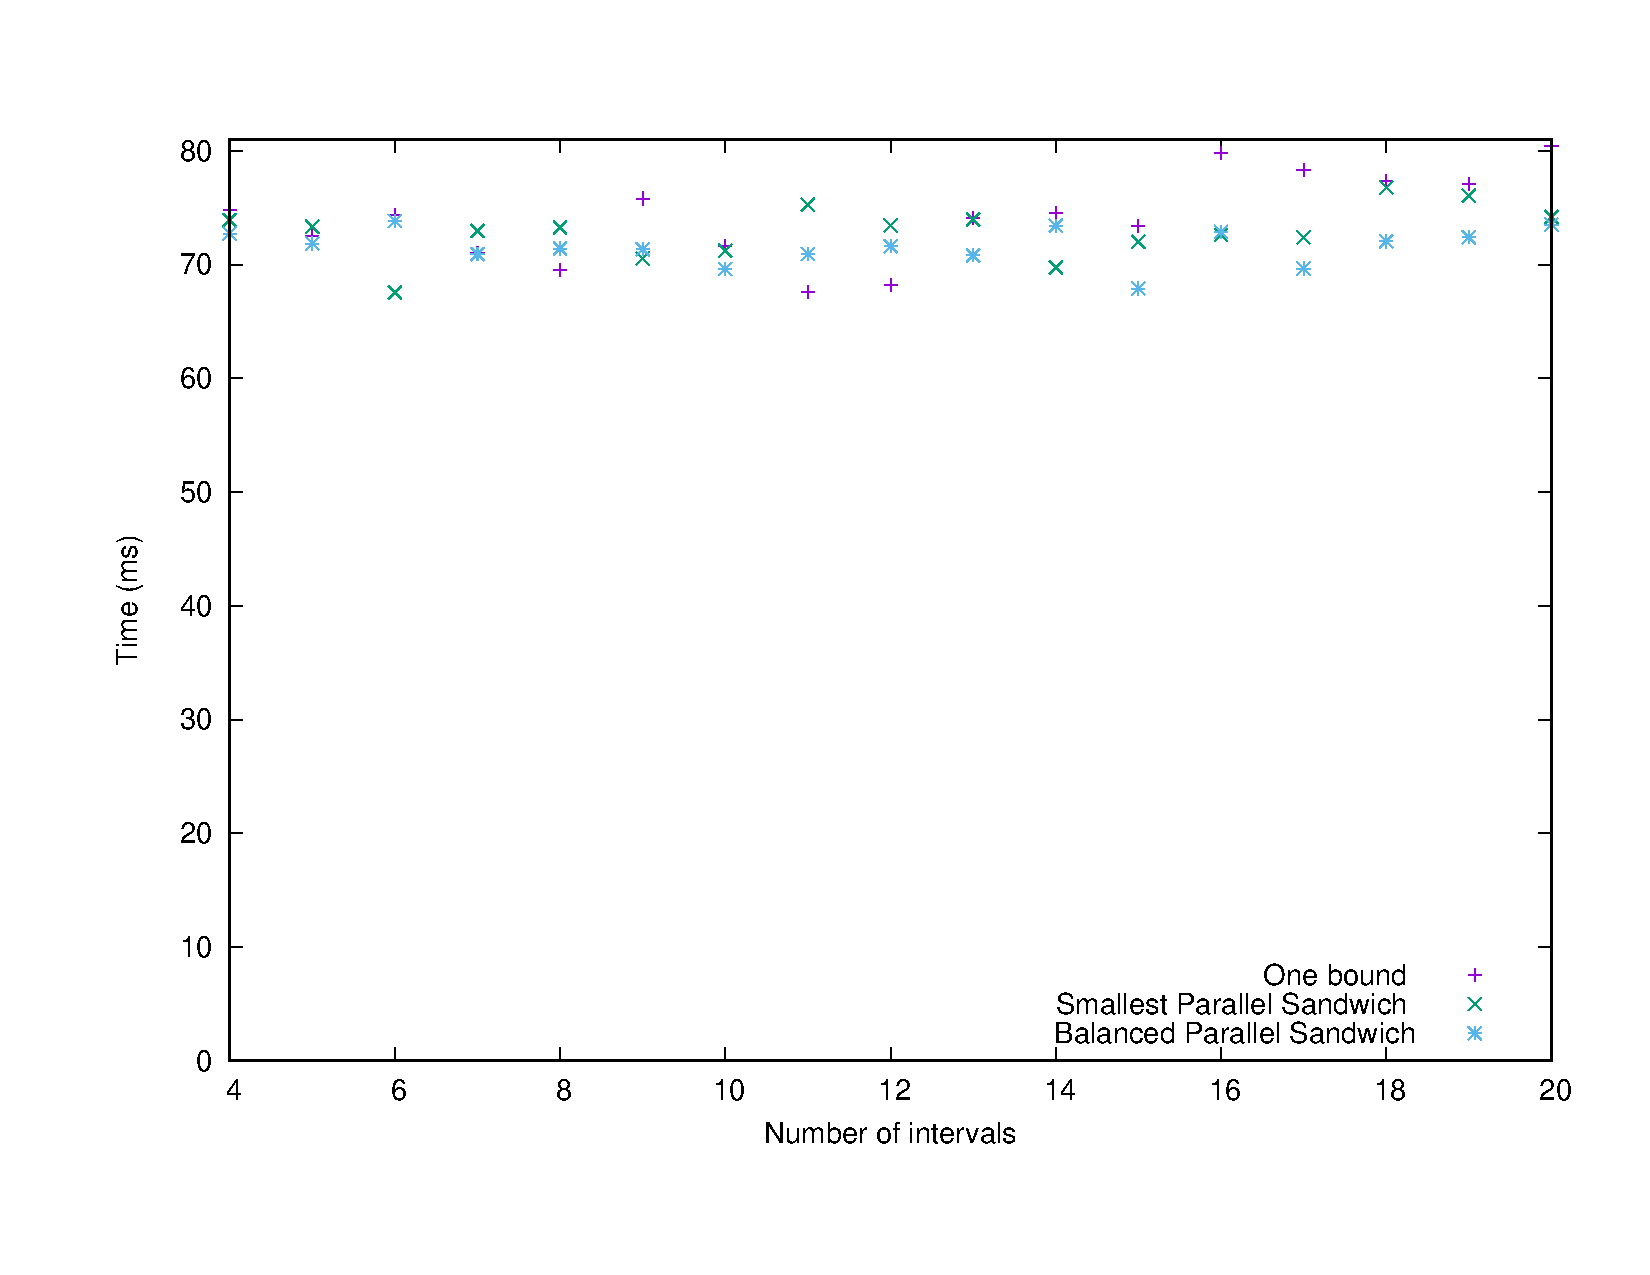
\includegraphics[scale=0.45]{timeshort.pdf}
 \caption{Evolution of average for $100$ simulations of $30,000$ events.}
\end{figure}

The trend of the curves on fig.~\ref{fig:intersshort} are notably similar to the curves of fig.~\ref{fig:interslong}. 
On the other hand, the three algorithm seems to run in a similar time on fig.~\ref{fig:timeshort}. Once again, this is due to the domination of the network time, which is the same for all algorithms, since the messages are all short.
On a single processor, the average time on $100$ simulations for $30,000$ events is to $23.06$ ms.
\todo{expliquer un peu plus, de toute facon on calcule tout les intervals en attendant le gars du debut vu que ca a tres peu de chance de coupler}

=======

\todo{Dire ce qui est utilisé comme techno entre les raspberry et donc la latence induite (à mesurer)}
>>>>>>> 43f1c719ccab17cdd0288dfaf16a9cd2cea56835

\subsection{Number of server used}
We now want to study the impact of the number of server used. As we noticed in fig.~\ref{fig:interslong}, there is an interessant point when the number of intervals is twice the number of servers (this threshold was observed for any number of servers between 2 and 7). We then look at the execution time of $100$ simulation from $2$ to $7$ servers, whith the \textsc{Balanced Parallel Sandwich} algorithm. The number of event $n$ of the simulation is set to $210,000$, and the number of intervals is always set to $2 \times \textrm{number of servers}$, since it is the first number at which the execution time of the algorithm starts to stagnate to it's lower value, for any number of processors.

\begin{figure}[H]
\centering
\label{fig:nbservs}
 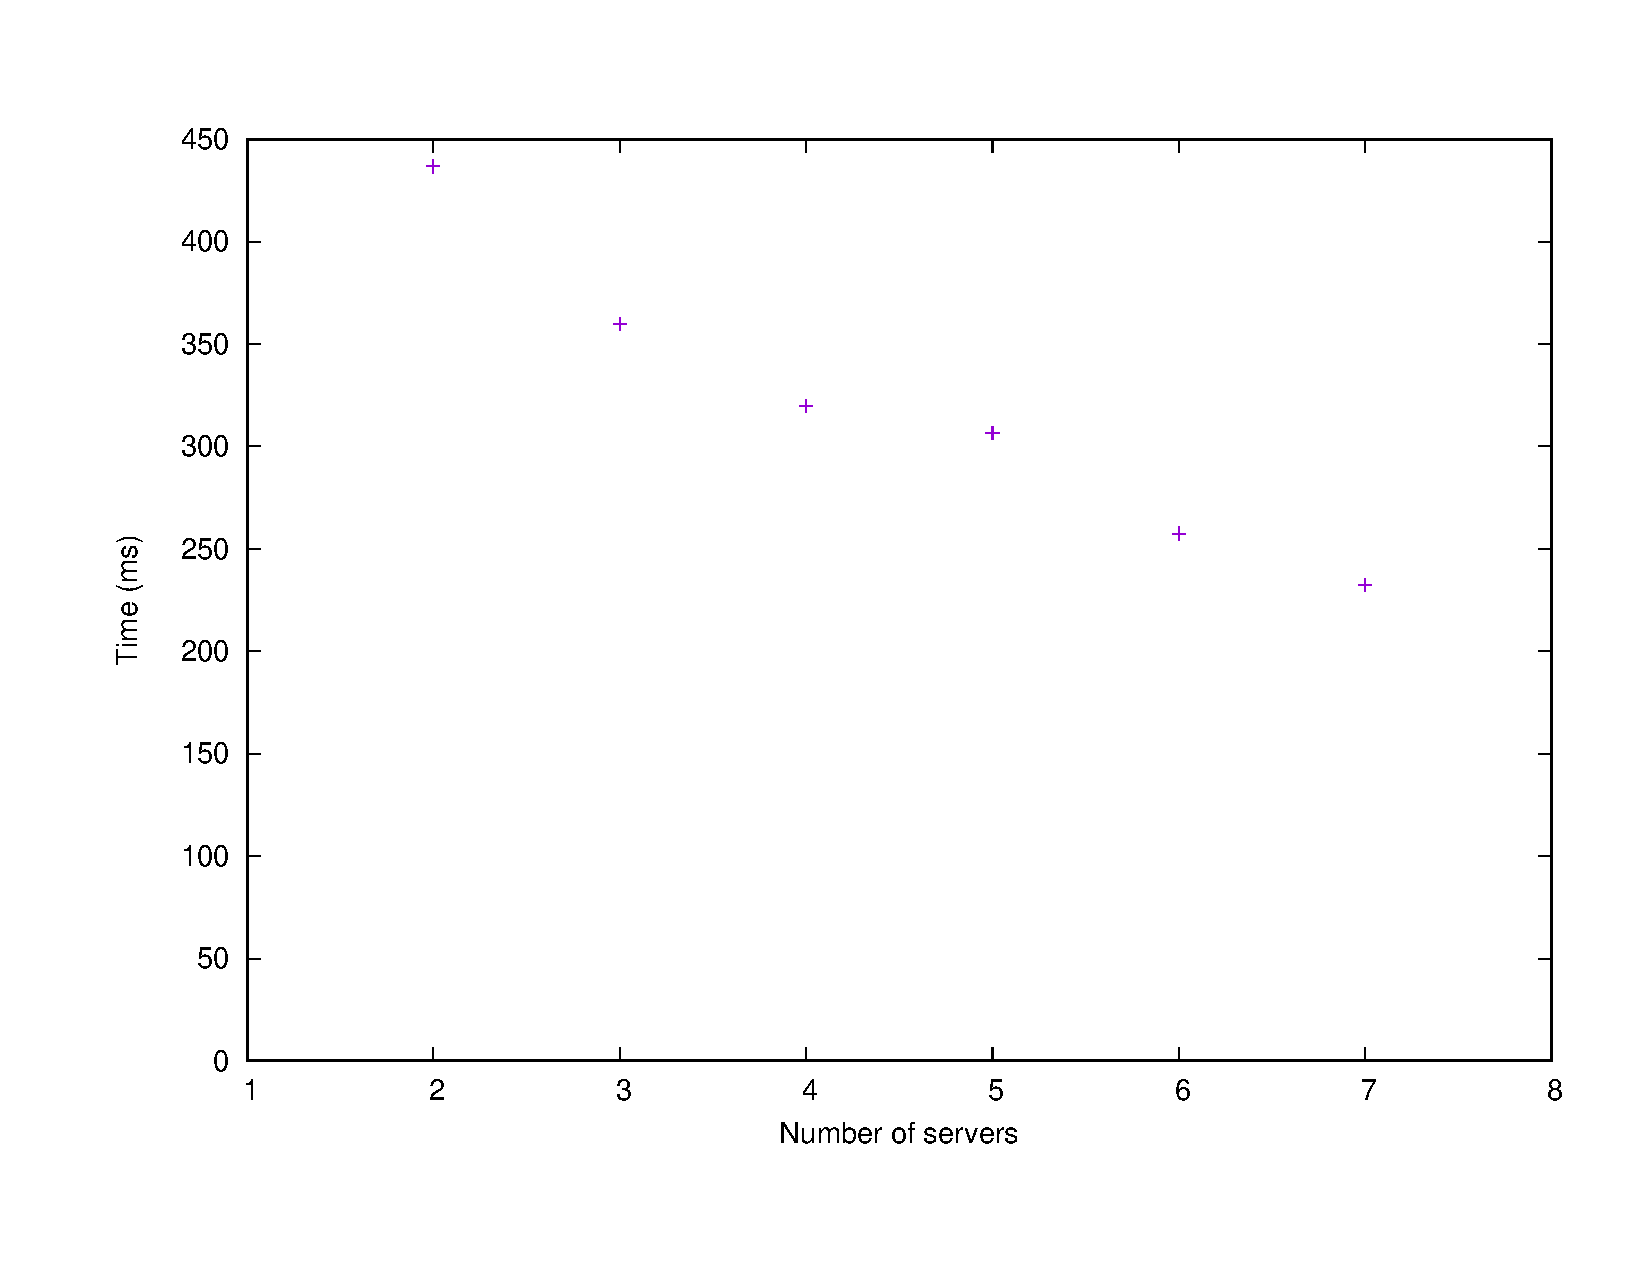
\includegraphics[scale=0.45]{numberofservers.pdf}
 \caption{Impact of the number of servers on the execution time.}
\end{figure}

As we can see on fig.\ref{fig:nbservs}, the more we have servers, the faster the algorithm runs.
\todo{bof cette conclusion, vu que c'est le reseau qui masque tout}

Practical problems: cost of the network transmission, especially for transmitting long sequences.
-> measure the time of a two way trip for a small message and the time of sending an interval.
To say that in practice we will not compute the whole sequence but statistic on it which could help
reduce the use of the network.


\bibliographystyle{plain}
\bibliography{biblio.bib}

\end{document}
